% ポストプロダクション段階で、エディターはカットやエフェクトなど様々な作業をしなくてはならない
In the post-production stage, an editor should do a lot of operations such as cutting scenes with mistakes, removing unexpected noise, applying audio and visual effects at appropriate timings, {\it etc}.
% それらの作業のために必要な情報は撮影時に発生するが、逐一ビデオと別途記録するのは面倒である
Most of information needed for the process, such as when an actor appeared in a scene, are shown during the shooting, however, we cannot note all of them with ordinary equipment.

\begin{figure}[htbp]
 \begin{center}
  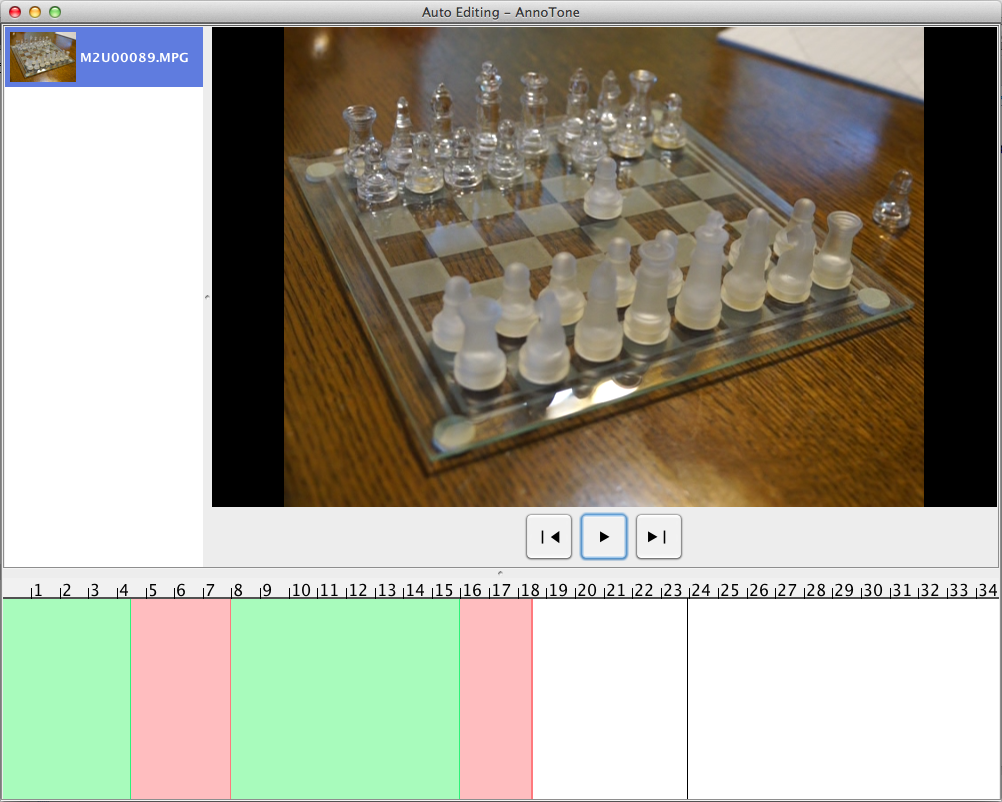
\includegraphics[width=80mm]{application_edit.png}
 \end{center}
 \caption{The user interface of our automatic video cutting application.}
 \label{fig:appl_map}
\end{figure}

% AnnoToneを使えば、そういう情報を録画中に埋め込んでおいて自動編集に使える
Using AnnoTone, we can embed that kind of information into a video in recording time, and conduct automatic editings after recording in accordance with the recorded annotations.
% 映像から失敗の部分を自動で切り取るとても簡単なアプリケーションを作成した。
We created a very simple video editing application as a sample of such usage, that automatically cut sections with mistakes off from a video using annotations that indicate ``Good'' or ``Bad'' at certain moments.
